\section{Image Captioning with RNNs and Attention}
\begin{frame}{}
    \LARGE Advanced Computer Vision: \textbf{Image Captioning with RNNs and Attention}
\end{frame}

\begin{frame}{Image Captioning with RNNs and Attention}

\only<1>{
\begin{figure}
\centering
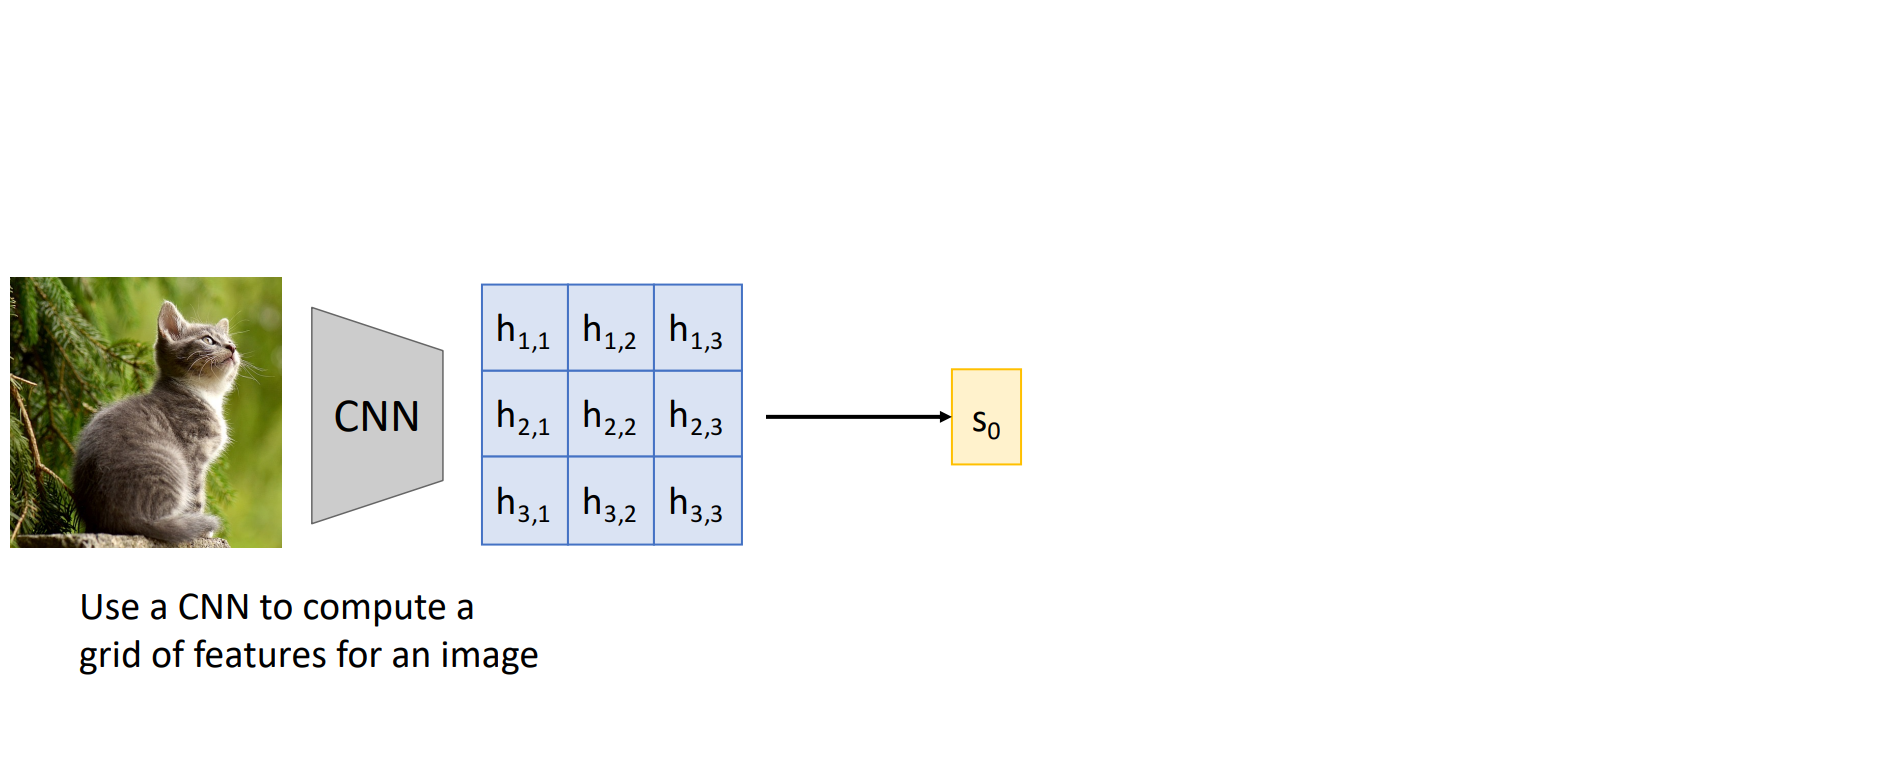
\includegraphics[width=1.0\textwidth,height=1.0\textheight,keepaspectratio]{images/advanced-cv/attention_10.png}
\end{figure}  
}

\only<2>{
\begin{figure}
\centering
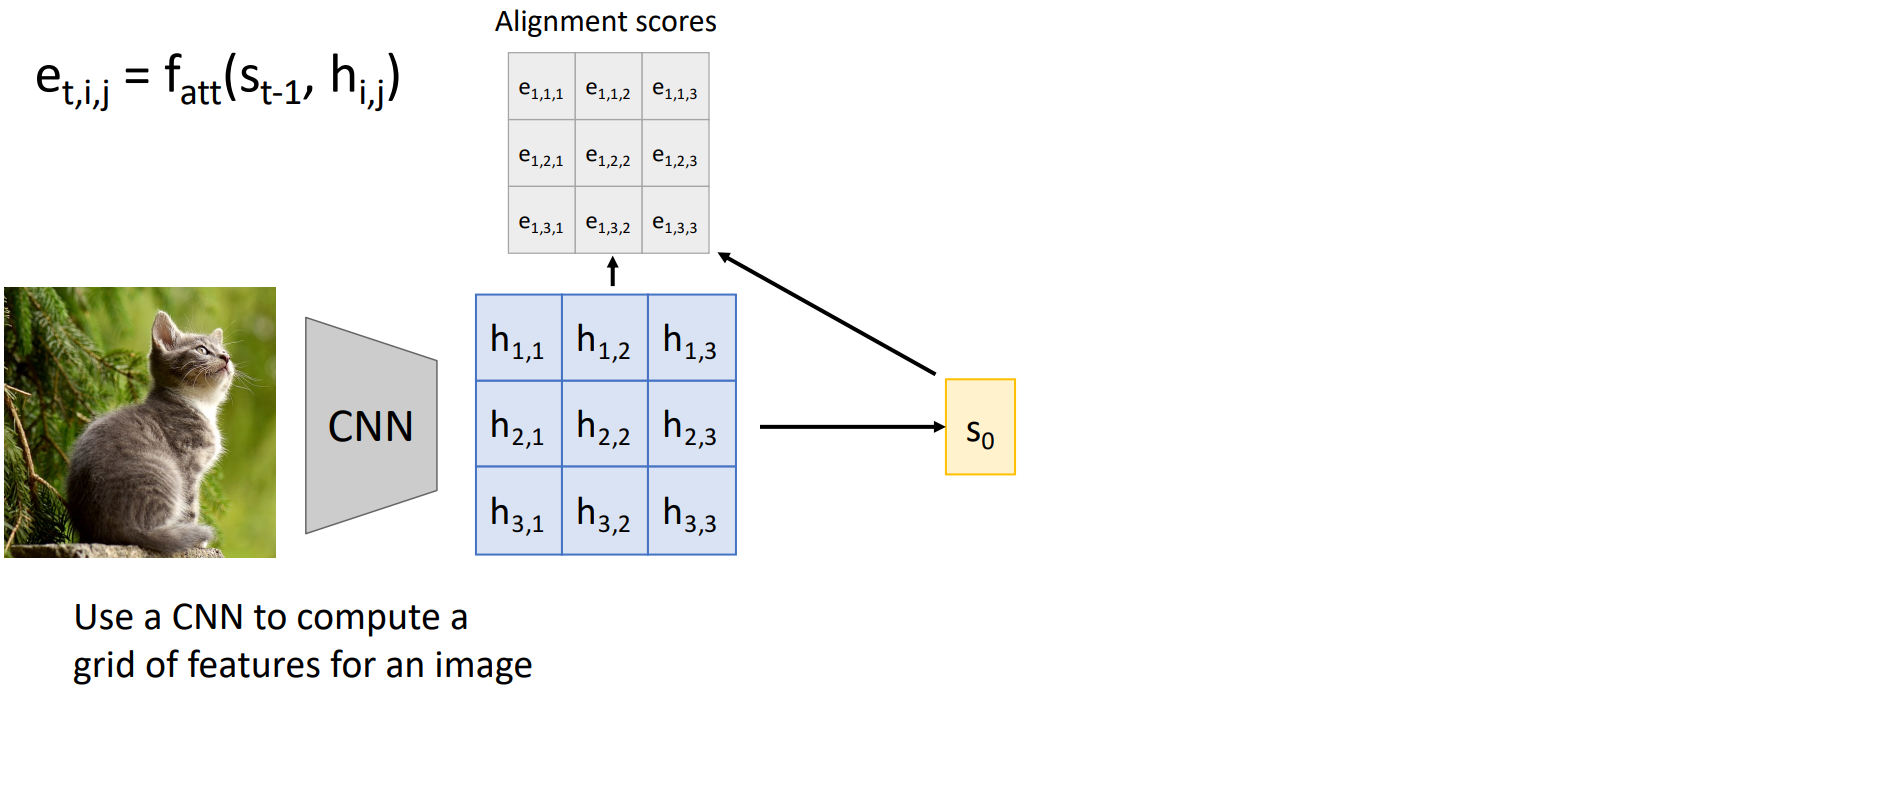
\includegraphics[width=1.0\textwidth,height=1.0\textheight,keepaspectratio]{images/advanced-cv/attention_11.png}
\end{figure}  
}

\only<3>{
\begin{figure}
\centering
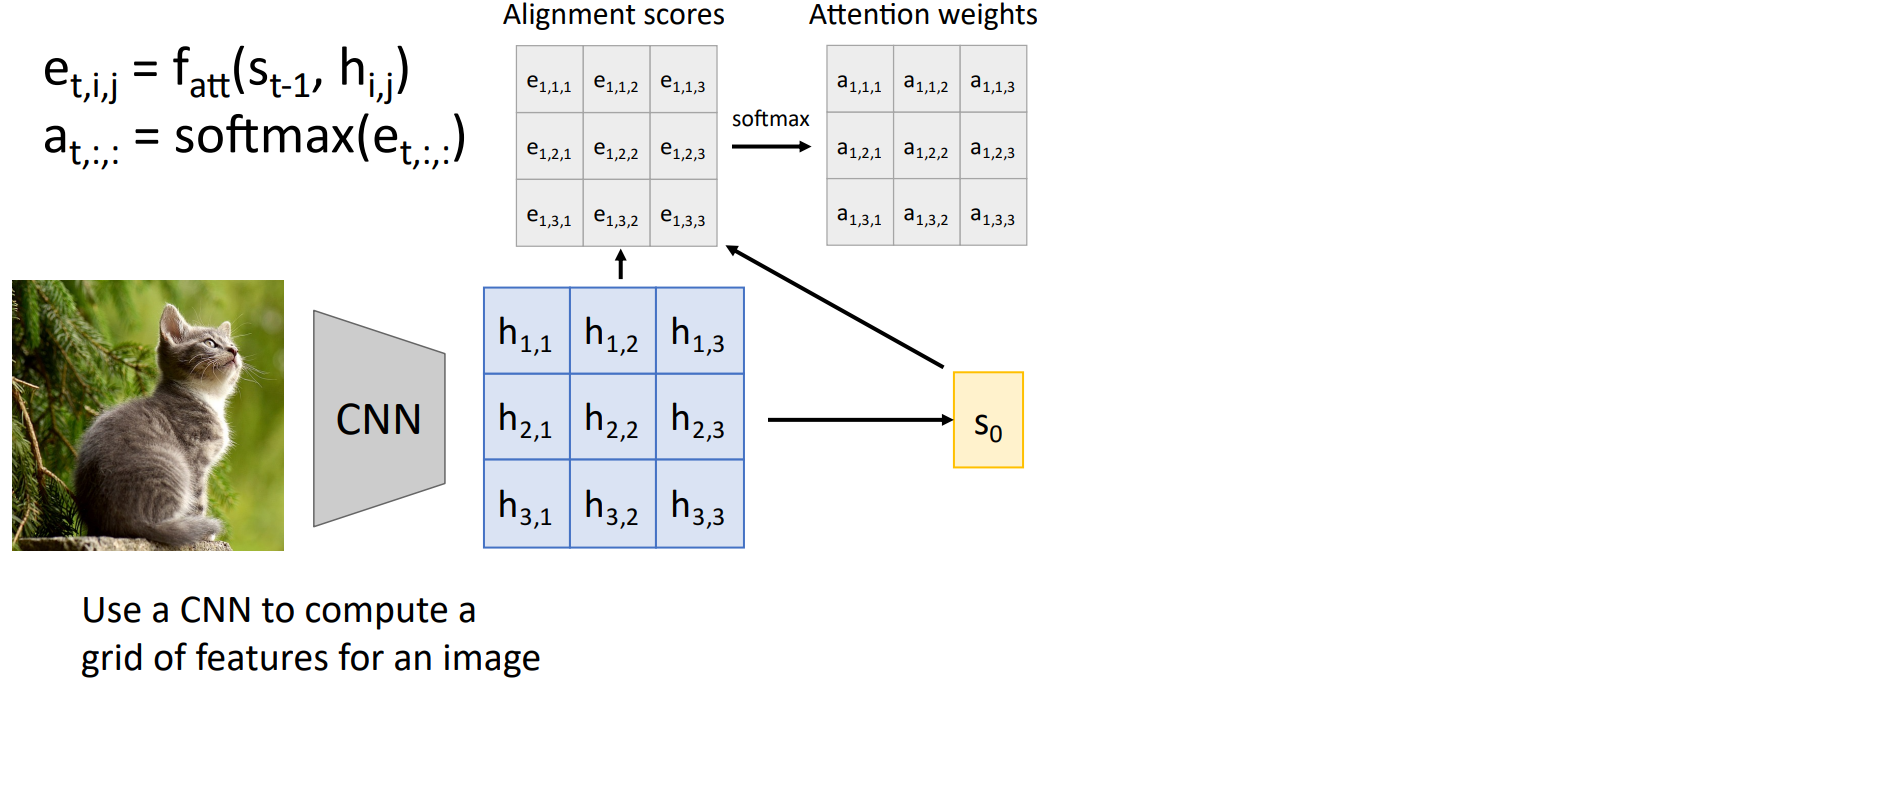
\includegraphics[width=1.0\textwidth,height=1.0\textheight,keepaspectratio]{images/advanced-cv/attention_12.png}
\end{figure}  
}

\only<4>{
\begin{figure}
\centering
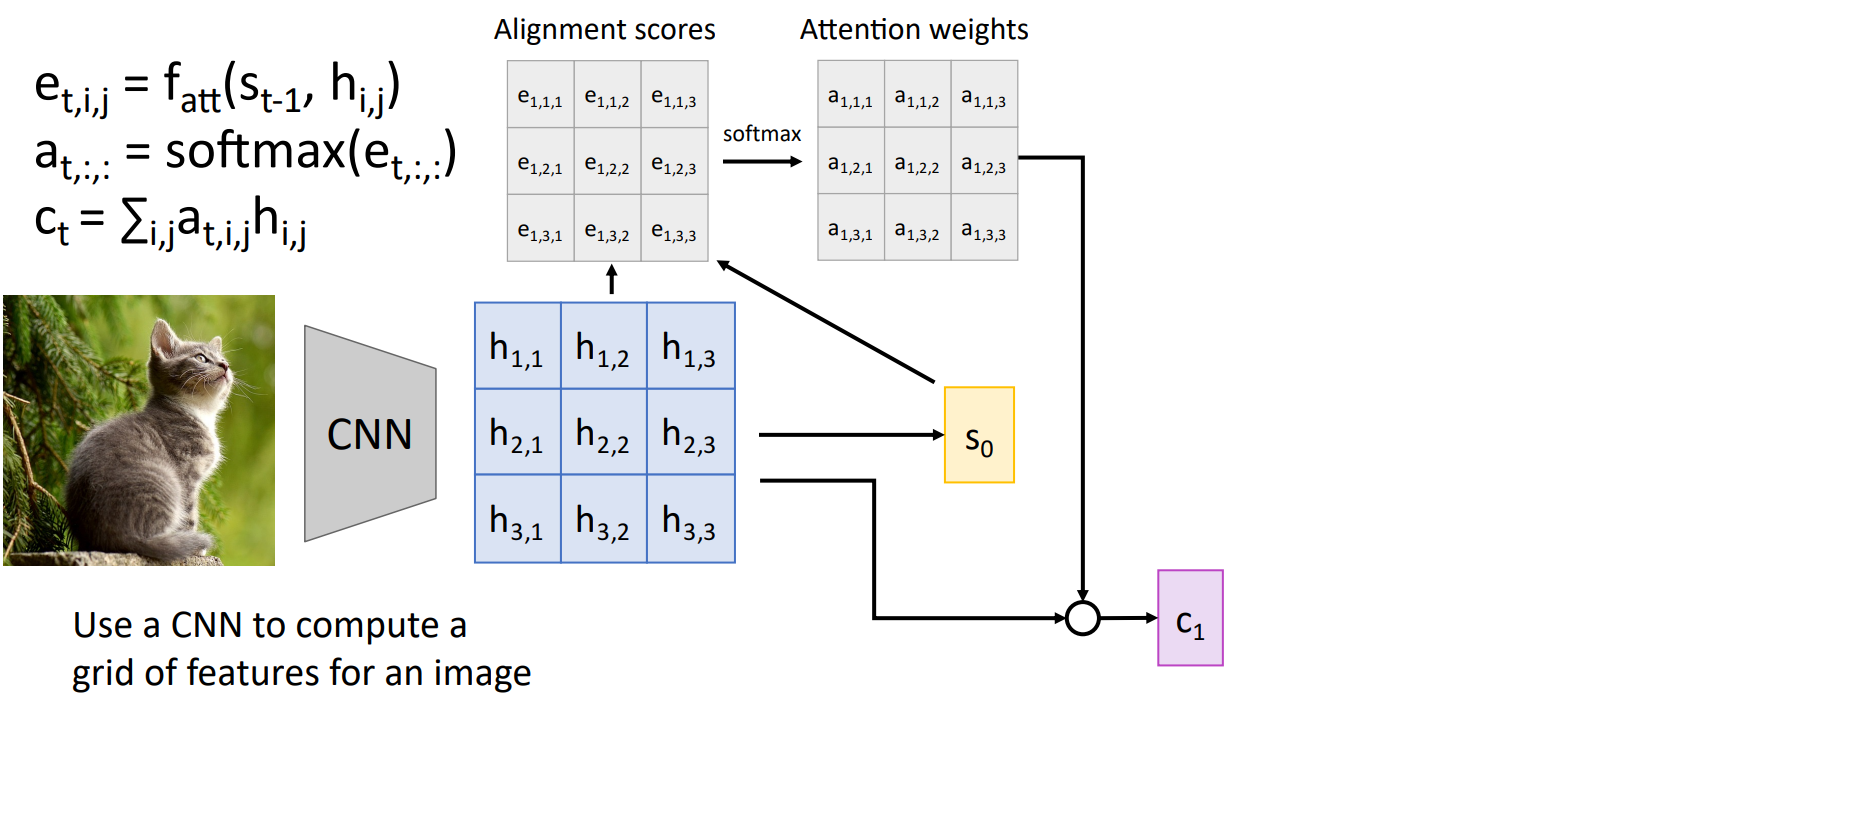
\includegraphics[width=1.0\textwidth,height=1.0\textheight,keepaspectratio]{images/advanced-cv/attention_13.png}
\end{figure}  
}

\only<5>{
\begin{figure}
\centering
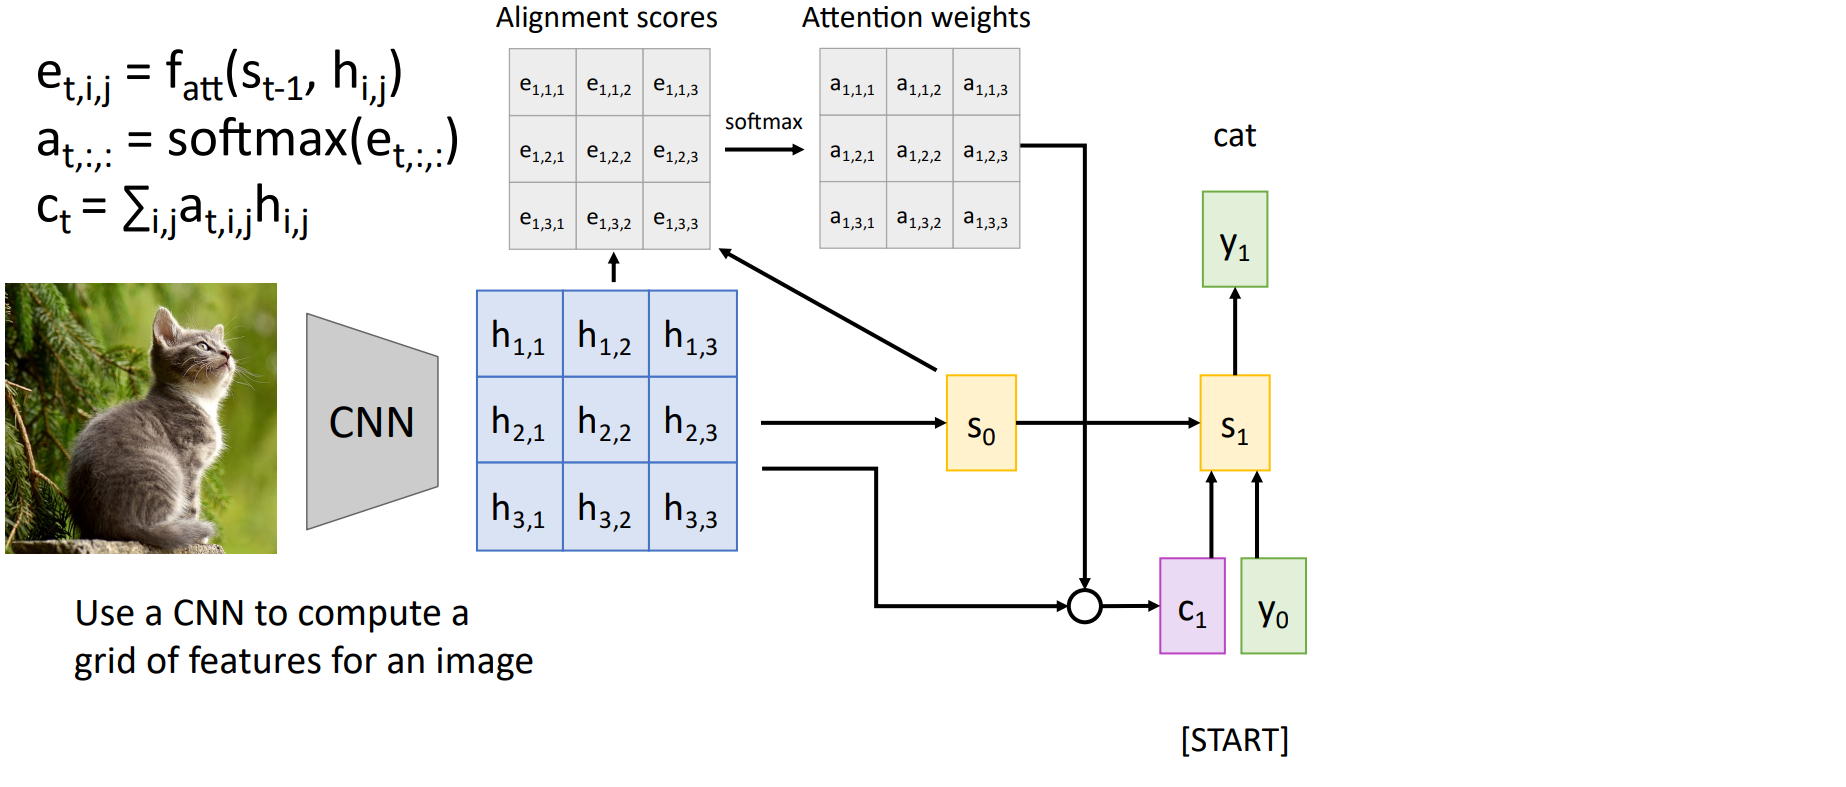
\includegraphics[width=1.0\textwidth,height=1.0\textheight,keepaspectratio]{images/advanced-cv/attention_14.png}
\end{figure}  
}

\only<6>{
\begin{figure}
\centering
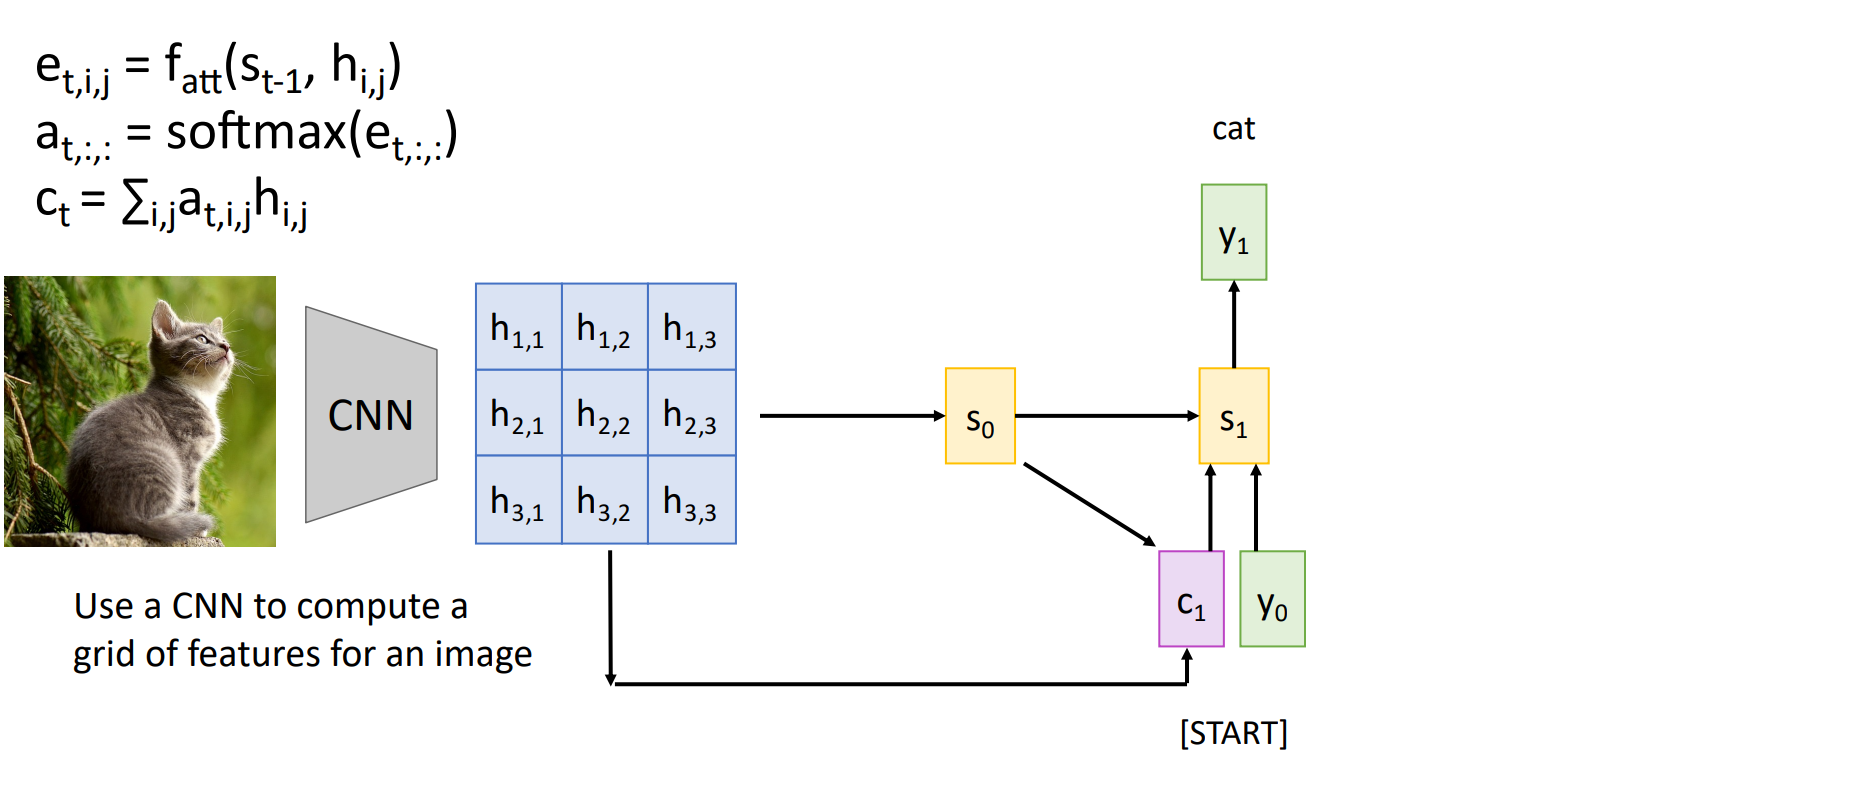
\includegraphics[width=1.0\textwidth,height=1.0\textheight,keepaspectratio]{images/advanced-cv/attention_15.png}
\end{figure}  
}

\only<7>{
\begin{figure}
\centering
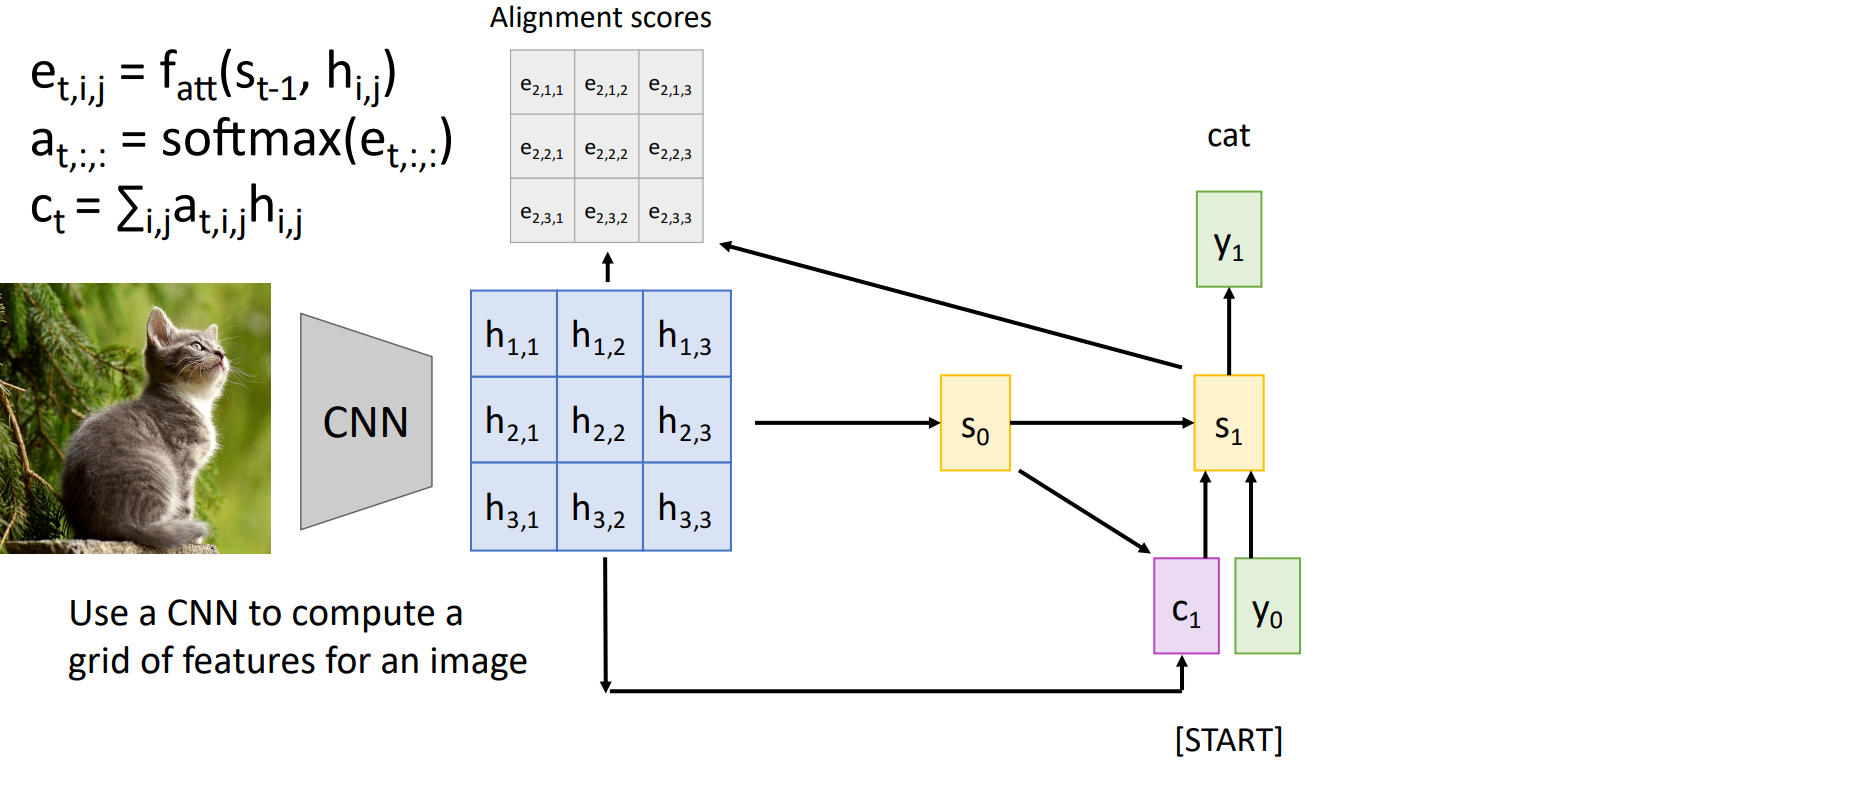
\includegraphics[width=1.0\textwidth,height=1.0\textheight,keepaspectratio]{images/advanced-cv/attention_16.png}
\end{figure}  
}

\only<8>{
\begin{figure}
\centering
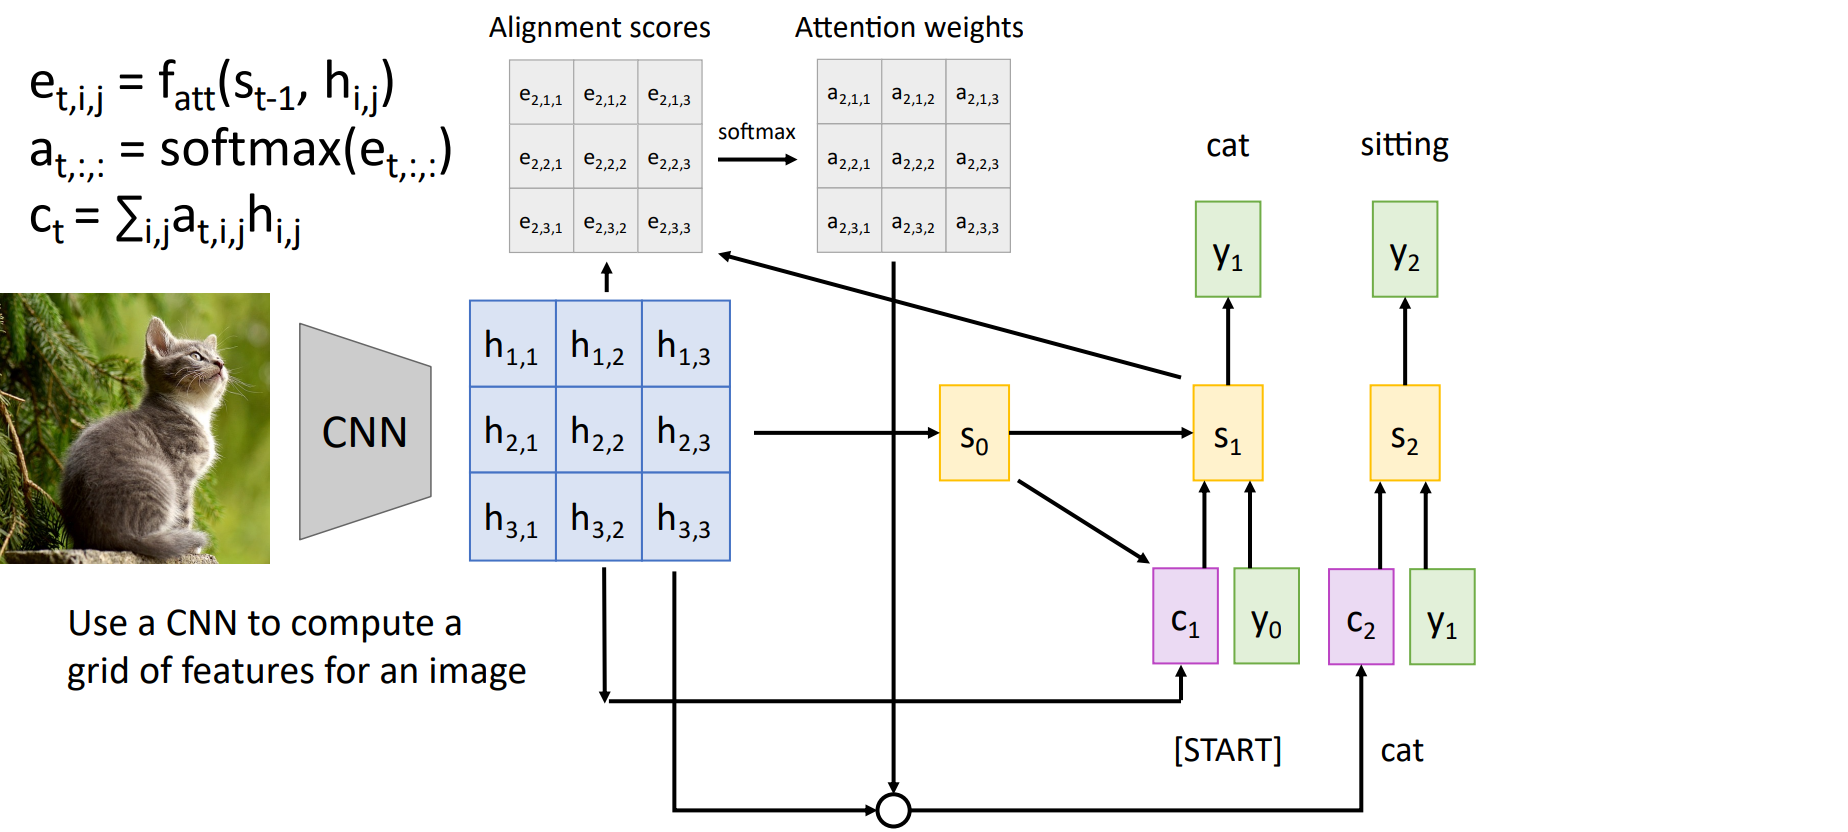
\includegraphics[width=1.0\textwidth,height=1.0\textheight,keepaspectratio]{images/advanced-cv/attention_17.png}
\end{figure}  
}

\only<9>{
\begin{figure}
\centering
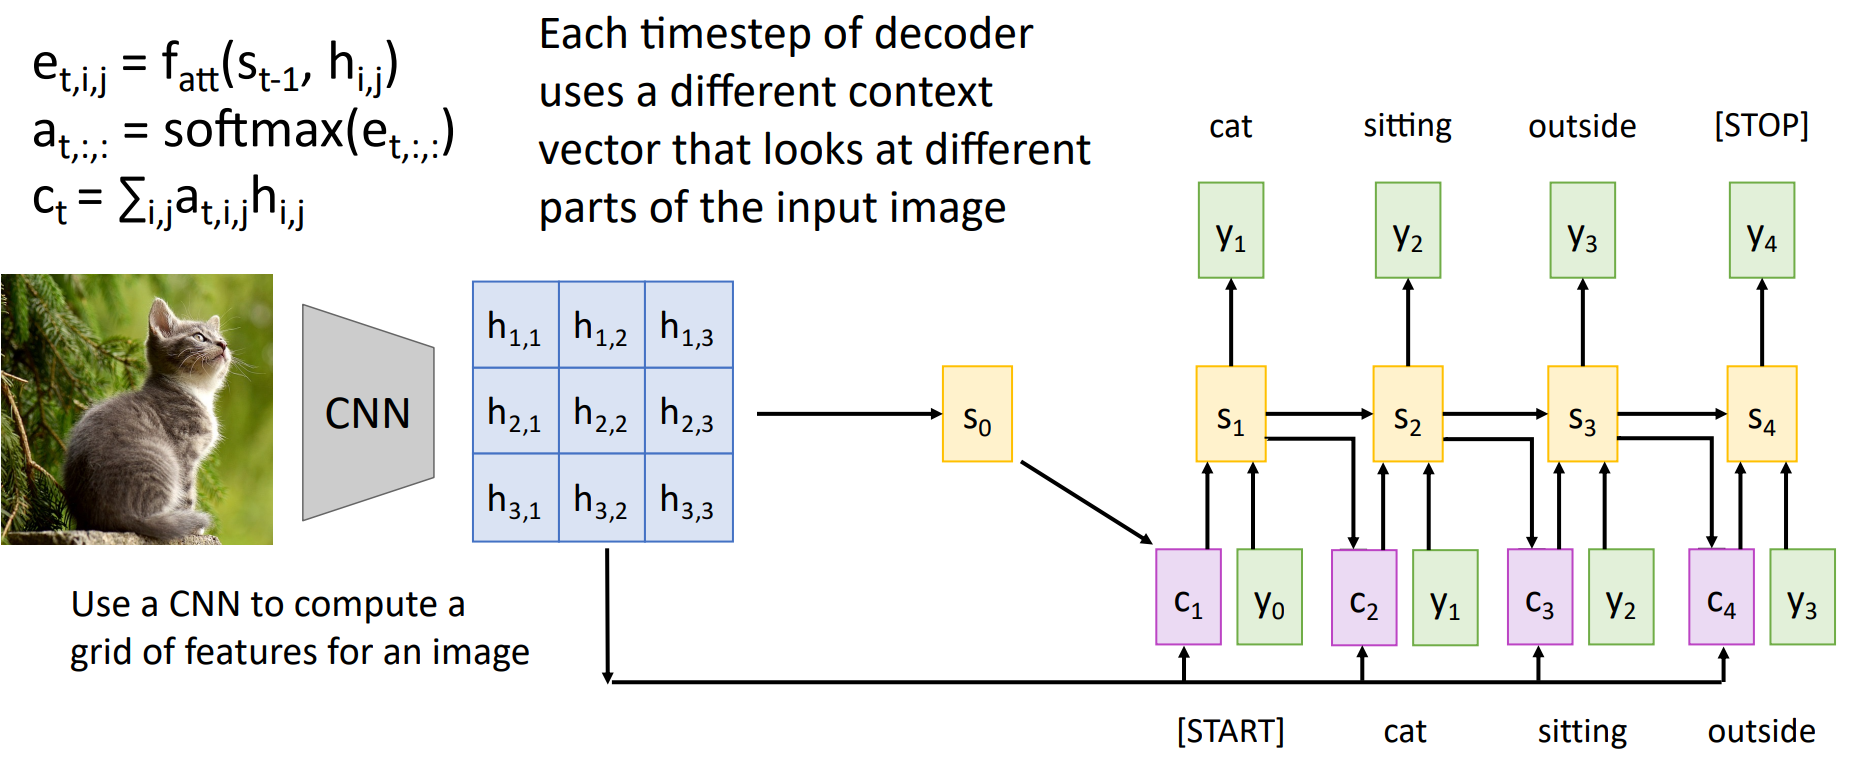
\includegraphics[width=1.0\textwidth,height=1.0\textheight,keepaspectratio]{images/advanced-cv/attention_18.png}
\end{figure}  
}

\only<10>{
\begin{figure}
\centering
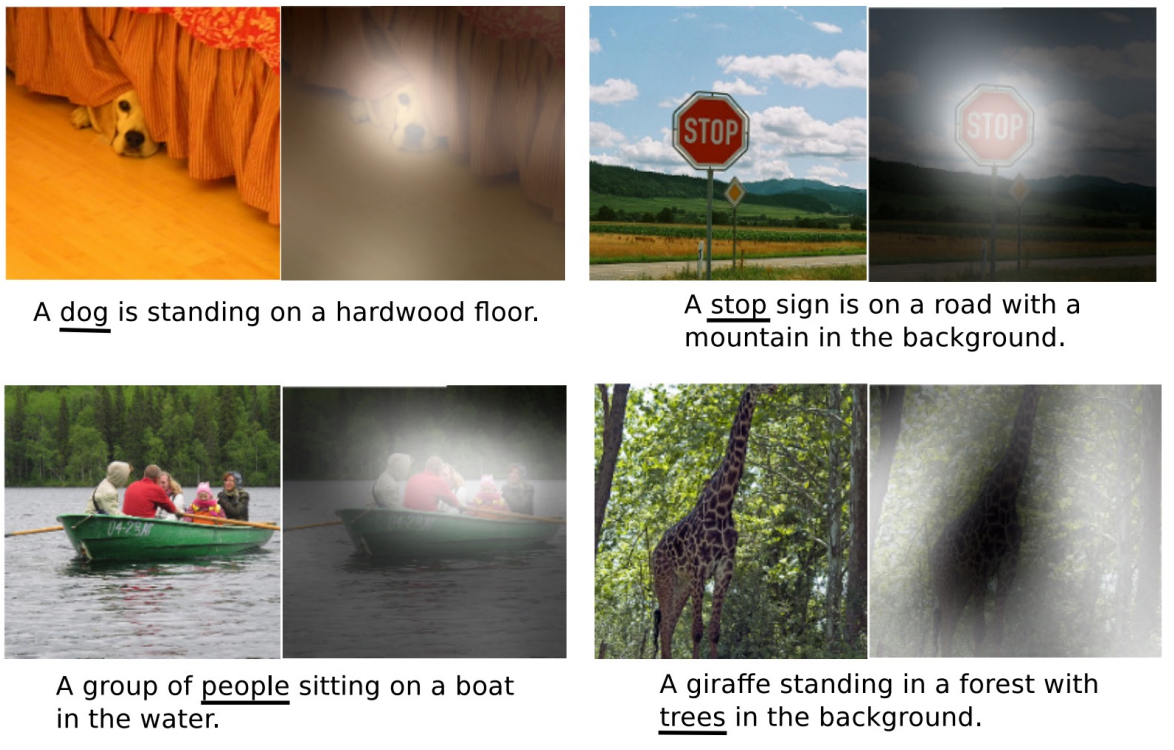
\includegraphics[width=1.0\textwidth,height=1.0\textheight,keepaspectratio]{images/advanced-cv/attention_19.png}
\end{figure}  
\footnotetext{Xu et al, “Show, AKend, and Tell: Neural Image CapAon GeneraAon with Visual AKenAon”, ICML 2015}
}

\end{frame}